\cleardoublepage

\chapter{Przegląd literatury}
W tym rozdziale zaprezentowano przegląd trzech różnych artykułów naukowych, opisujących podejścia do testowania i ewaluacji dużych modeli językowych wykorzystywanych w systemach RAG. Pierwsze dwie publikacje oparte są na danych nieustrukturyzowanych, podczas gdy ostatnia skupia się na danych ustrukturyzowanych.
    

    \section{Benchmark MEBench}
    W artykule \enquote{MEBench: Benchmarking Large Language Models for Cross-Document Multi-Entity Question Answering} \cite{art1_2025} autorzy przedstawili MEBench, czyli skalowalny wielodokumentowy test wydajnościowy (ang. \textit{benchmark}). Zaprojektowany został do systematycznej ewaluacji systemów LLM zdolnych do wyszukiwania, łączenia informacji i wyciągania wniosków z rozproszonych i bogatych w treść zewnętrznych źródeł danych. Benchmark składa się z 4780 pytań podzielonych na trzy kategorie wnioskowania \ref{mebench_kategorie_pytan}: porównawcze, relacyjne i statystyczne. 

    \begin{table}[h]
        \centering
        \caption{ Definicja trzech kategorii pytań wchodzących w skład frameworka MEBench }
        \begin{tabularx}{\textwidth}{|p{5cm}|X|}
        \hline
        \textbf{Kategoria pytań} & \textbf{Definicja} \\
        \hline
        Wnioskowanie porównawcze & Umożliwia sprawdzenie czy LLM jest w stanie zestawić ze sobą elementy z różnorodnych źródeł danych zachowując ich spójność i zapewniając syntezę kontekstową.  \\ \hline
        
        Wnioskowanie relacyjne & Pozwala zbadać zdolność modelu do odwzorowania relacji i przeciwstawnych faktów pomiędzy dokumentami.  \\ \hline
        
        Wnioskowanie statystyczne & Umożliwia testowanie kompetencji LLMa w syntezie ilościowej obejmującej analizę korelacji, analizę wariancji, analizę rozkładu oraz agregację. \\ \hline
        \end{tabularx}
        \label{mebench_kategorie_pytan}
    \end{table}
    
    \noindent Dodatkowo, każda z nich dzieli się na typy (podkategorie), których jest łącznie osiem. Takie podziały umożliwiają symulowanie rzeczywistych scenariuszy zapytań, pokrywających rozproszone informacje przypisane do dedykowanych źródeł danych. Na poniższym rysunku \ref{benchmarks_vs_mebench} zwizualizowano porównanie dostępnych na rynku benchmarków z MEBench. Jak można zauważyć, w przeciwieństwie do konkurencji, testuje on LLMy i systemy RAG bez ignorowania ani jednego załączonego dokumentu.

    \begin{center}
        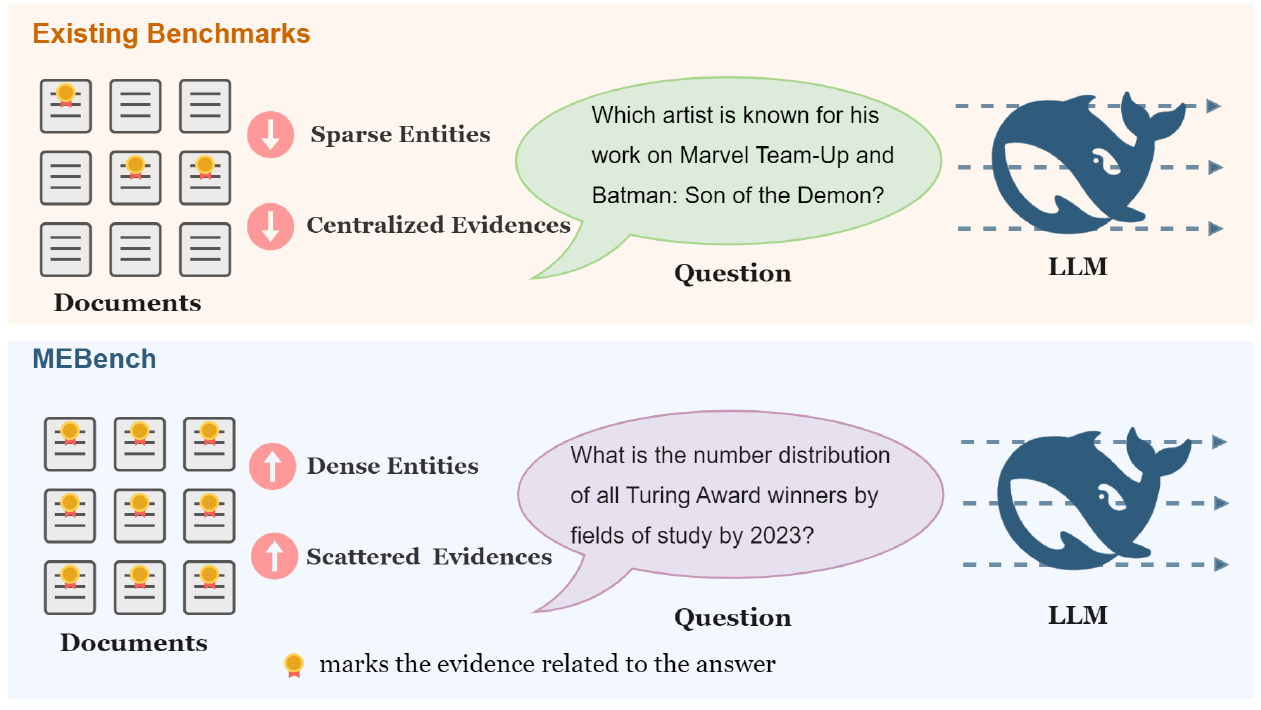
\includegraphics[width=0.6\textwidth]{rysunki/benchmarks_vs_mebench.png}
        \captionof{figure}{ Porównanie istniejących benchmarków z MEBench \cite{art1_2025}}
        \label{benchmarks_vs_mebench}
    \end{center}

    Schemat (ang. \textit{pipeline}) budowania benchmarku MEBech składa się z trzech etapów. Pierwszym z nich jest zebranie niezbędnych dokumentów. Duży model językowy GPT-4 pobiera dokumenty z Wikipedii za pomocą dedykowanego API. Dotyczą one pewnego obszaru wiedzy. W następnym kroku, zwanym ekstrakcją informacji, te dane są przetwarzane za pomocą małego modelu językowego (SLM) tak, aby na ich podstawie uzyskać ustrukturyzowaną bazę danych. Ostatnim krokiem jest generowanie pytań i odpowiedzi. Pytania są tworzone za pomocą LLMa na podstawie predefiniowanego szablonu (struktury). Następnie, model przekształca je z języka naturalnego na kwerendy bazodanowe. Na podstawie wyników tych zapytań tworzone są odpowiedzi w języku naturalnym. Poprawność odpowiedzi jest gwarantowana dzięki programowej weryfikacji, a nie na podstawie wiedzy modelu. Tak przygotowane pytania i odpowiedzi zapisywane są do oddzielnej bazy danych, którą wykorzystuje się do testów modeli. Na poniższym rysunku \ref{mebench_pipeline}, autorzy omawianego artykułu szczegółowo zaprezentowali przebieg tworzenia frameworka MEBench na przykładzie danych dotyczących członków ACM (ACM Fellows).
    
    \begin{center}
        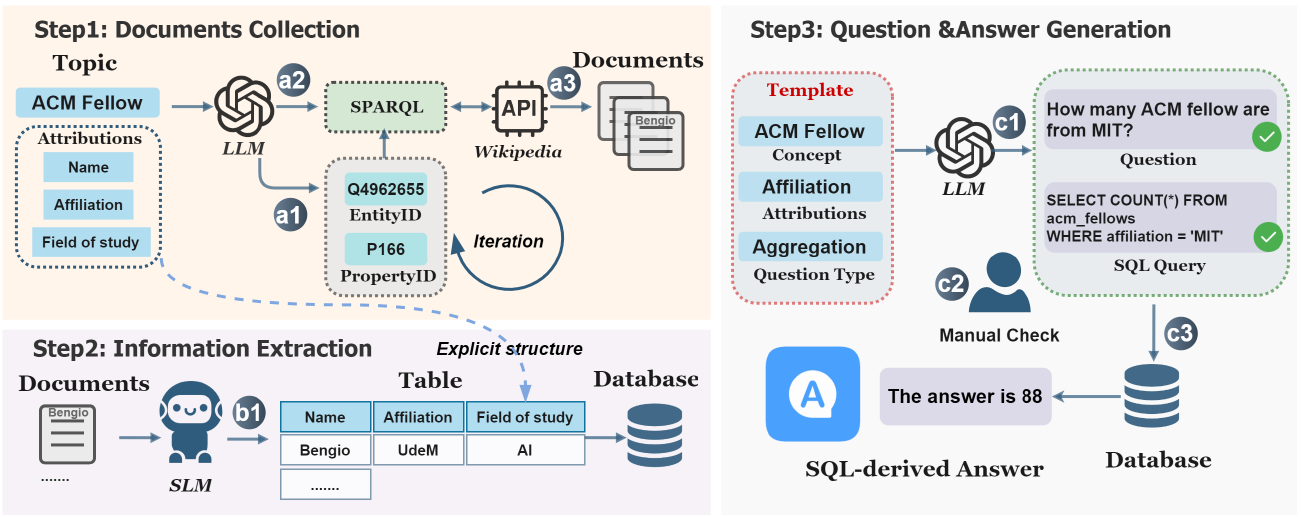
\includegraphics[width=0.85\textwidth]{rysunki/mebench_pipeline.png}
        \captionof{figure}{ Schemat tworzenia benchmarku MEBench \cite{art1_2025}}
        \label{mebench_pipeline}
    \end{center}

    Benchmark składa się 4780 pytań, które podzielone są na 3406 pytań treningowych i 1374 pytań testujących. Zebrane dane dzielone są na trzy grupy bazując na ich złożoności — mało, średnio i bardzo złożone. Do badań użyto otwartoźródłowego modelu Llama-3-Instruct (oznaczonego z dopiskiem FT) oraz zamknięte (komercyjne) modele: GPT-3.5-turbo i GPT-4. Warto podkreślić, że pytania treningowe są  wykorzystywane tylko do dostrojenia otwartoźródłowego LLMa. Wszystkie modele poddano ewaluacji w dwóch wariantach: bazowym, opierającym się wyłącznie na wiedzy parametrycznej oraz rozszerzonym o system RAG. Poniższy rysunek \ref{mebench_accuracy} przedstawia porównanie skuteczności odpowiedzi modeli, mierzonej jako dokładność (ang. \textit{accuracy}).

    \begin{center}
        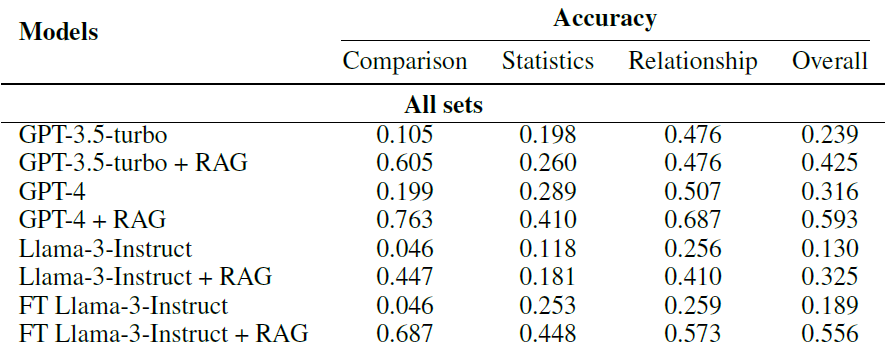
\includegraphics[width=0.75\textwidth]{rysunki/mebench_accuracy.png}
        \captionof{figure}{ Skuteczność modeli językowych w benchmarku MEBench z podziałem na kategorie pytań testowych \cite{art1_2025}}
        \label{mebench_accuracy}
    \end{center}

    Na podstawie wyników można wywnioskować, iż system GPT-4 + RAG osiągnął najwyższą dokładność wynoszącą 59,3\%. W szczególności, najlepiej poradził sobie w pytaniach porównawczych i relacyjnych. Na drugim miejscu uplasował się model FT Llama-3-Instruct z wynikiem 55,6\%. Na tle innych, najbardziej wyróżnił się w kontekście pytań statystycznych. Pytania te w ogólności stanowiły największe wyzwanie dla badanych systemów, co skutkowało najmniej satysfakcjonującymi wynikami. MEBench skutecznie wskazuje niedociągnięcia obecnych modeli LLM, ale także stanowi motywację do rozwoju solidnych architektur systemów QA, które precyzyjnie uwzględniają specyfikę zróżnicowanych zestawów danych.


    \section{Benchmark RGB}
    Drugim omawianym artykułem jest \enquote{Benchmarking Large Language Models in Retrieval-Augmented Generation} \cite{art2_unstructured2024}. Autorzy tej pracy przeanalizowali skuteczność różnych dużych modeli językowych działających w ramach systemu RAG, gdzie zewnętrznym źródłem wiedzy były dane nieustrukturyzowane. Testy przeprowadzono odpytując LLMy łącznie tysiącem pytań z czterech podstawowych kategorii: odporność na szum, odmowa odpowiedzi, integracja informacji oraz odporność na błędne fakty. W poniższej tabeli \ref{rgb_kategorie_pytan} zdefiniowano każdą z nich.

    \begin{table}[h]
        \centering
        \caption{ Definicja czterech kategorii pytań tworzących benchmark RGB }
        \begin{tabularx}{\textwidth}{|p{4.5cm}|X|}
        \hline
        \textbf{Kategoria pytań} & \textbf{Definicja} \\
        \hline
        Odporność na szum (ang. \textit{noise robustness}) & Umożliwia sprawdzenie czy LLM potrafi wydobywać użyteczne informacje z zaszumionych dokumentów.  \\ \hline
        
        Odmowa odpowiedzi (ang. \textit{negative rejection}) & Pozwala zbadać czy LLM odmówi odpowiedzi na pytanie, kiedy nie ma wystarczającej ilości danych na konkretny temat w żadnym dokumencie.  \\ \hline
        
        Integracja informacji (ang. \textit{information integration}) & Służy do sprawdzenia czy LLM jest w stanie odpowiedzieć na złożone pytania wymuszające zebranie i połączenie ze sobą informacji z wielu dokumentów. \\ \hline

        Odporność na błędne fakty (ang. \textit{counterfactual robustness}) & Umożliwia sprawdzenie czy LLM potrafi wskazać błędne fakty w dokumentach bazując na swojej wiedzy parametrycznej. W wiadomości systemowej modelu powinno być wspomniane, że dokumenty mogą zawierać błędy. \\ \hline
        \end{tabularx}
        \label{rgb_kategorie_pytan}
    \end{table}

    \noindent W celu przeprowadzenia testów, autorzy utworzyli test wydajnościowy Retrieval-Augmented Generation Benchmark (RGB). Jest to najnowszy framework do ewaluacji systemu RAG dla języka angielskiego i chińskiego. RGB jest podzielony na cztery oddzielne zestawy testów. Każdy z nich odpowiada wyżej wymienionym kategoriom pytań, które są zadawane sześciu ówcześnie najnowocześniejszym modelom językowym: GPT-3.5-turbo, ChatGLM-6B, ChatGLM2-6B, Vicuna-7b-v1.3, Qwen-7B-Chat oraz BELLE-7B-2M.

    W celu wygenerowania pytań i odpowiedzi do przypadków testowych w benchmarku, bazując na najaktualniejszych źródłach danych z internetu, stosuje się ChatGPT. Na podstawie zewnętrznych dokumentów tworzy on krótkie opisy najważniejszych wydarzeń, pytania i odpowiedzi. Tak utworzone treści są ręcznie filtrowane przez twórców. Pytania są dzielone na opisane wcześniej cztery różne grupy. Dla każdego zapytania zostaje użyte API Google do zaciągnięcia dziesięciu istotnych stron internetowych. Te zewnętrzne dokumenty są następnie dzielone na pozytywne i negatywne w zależności od tego czy zawierają odpowiedź czy nie. Dopiero ten zaciągnięty zbiór dokumentów służy jako zewnętrzna wiedza modelu w systemie RAG.

    Ewaluację modeli językowych przeprowadzono oddzielnie dla każdego z czterech zestawów testowych. Poniższy rysunek \ref{rgb_4_kategorie_pytan} prezentuje przykład pytań i odpowiedzi z każdej kategorii.

    \begin{center}
        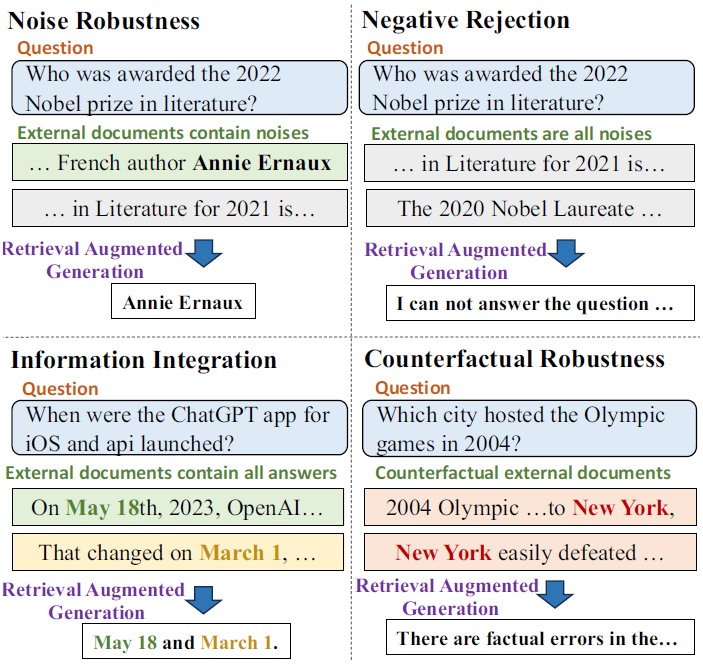
\includegraphics[width=0.6\textwidth]{rysunki/rgb_4_kategorie_pytan.png}
        \captionof{figure}{ Przykład pytań i odpowiedzi dla czterech zestawów testowych służących do ewaluacji systemów RAG w ramach benchmarku RGB \cite{art2_unstructured2024}}
        \label{rgb_4_kategorie_pytan}
    \end{center}

    \noindent W wynikach pierwszego testu zauważono, że LLMy wykazały się dużą zdolnością odfiltrowania istotnych informacji z zaszumionych danych, czyniąc RAG obiecującą techniką rozszerzającą zdolności modeli językowych. Natomiast, gdy stopień zaszumienia przekroczył 80\%, dokładność odpowiedzi modeli znacząco spadła, o około 15\% dla każdego z nich. W tym podejściu ChatGPT osiągnął najlepsze wyniki. W drugim teście dostrzeżono, że odmowa odpowiedzi modeli stanowi największe wyzwanie. Najwyższym wskaźnikiem odmowy odznaczył się model GPT ze skutecznością 45\%. Odnośnie pytań z trzeciej kategorii, modele poradziły sobie nieco lepiej. Najwyższą skutecznością integracji informacji wykazał się model Qwen na poziomie 67\%. Jak łatwo zauważyć, pytania z tej dziedziny także stanowią duże wyzwanie dla modeli językowych. Dla pytań z ostatniej grupy testowej, ChatGPT poradził sobie najlepiej. Wykazał się on znajomością faktów bazując tylko na wewnętrznej parametrycznej wiedzy na poziomie 91\%. Natomiast, przy dołączonych zewnętrznych dokumentach zawierających przeciwstawne fakty, wykazał się on już skutecznością na poziomie 17\%, co i tak okazało się być najlepszym wynikiem. Rezultaty eksperymentów dla benchmarku RGB wskazują, że LLMy mają ograniczenia dla każdej z czterech kategorii pytań. Dowodzi to, że aby zapewnić dokładne i wiarygodne odpowiedzi dużych modeli językowych kluczowe jest zachowanie ostrożności i staranne projektowanie systemów RAG.
    

    \section{Benchmark NL-to-SQL} 

    W artykule \enquote{Benchmarking Large Language Models for NL-to-SQL: A Comprehensive Evaluation of Accuracy, Cost and Throughput} \cite{art3_structured2024} autorzy skupili się na rozwoju benchmarku pozwalającego na ewaluację dużych modeli językowych w kontekście systemu RAG, gdzie zewnętrznym źródłem ustrukturyzowanych danych jest baza danych SQL. Sprawdzono jak modele radzą sobie z zamianą języka naturalnego na kwerendy bazodanowe (NL-to-SQL). Przetestowano LLMy na różnych platformach za pomocą łącznie 360 pytań selektywnie wybranych ze zbioru danych BIRD \cite{bird2018}. Były to kwerendy o następujących poziomach zaawansowania: łatwe, umiarkowane i trudne \cite{3_levels_of_questions_difficulty2023}. Poziom trudności zdefiniowano na podstawie liczby komponentów SQL, selekcji oraz warunków, tak aby zapytania zawierające większą liczbę słów kluczowych SQL były uznawane za trudniejsze. Na sześciu różnych platformach hostingowych przebadano łącznie 30 modeli (niektóre z nich się powtarzały). Poniżej w tabeli \ref{nltosql_modele} wypisano wszystkie z nich.    

    \begin{table}[h]
        \centering
        \caption{ Platformy i przypisane do nich LLMy badane w ramach benchmarku NL-to-SQL \cite{art3_structured2024}}
        \begin{tabularx}{\textwidth}{|p{3cm}|X|}
        \hline
        \textbf{Platforma} & \textbf{Modele LLM} \\
        \hline
        Anyscale & Llama3-70B, Llama2-70B, Mistral 7B (Version 1), Mixtral8x7B, CodeLlama-70B  \\ \hline
        
        Amazon Bedrock & Llama3-70B, Llama2-70B, Mistral-7B (Version 2), Mixtral8x7B, Claude3-Sonnet, Claude3-Haiku  \\ \hline
        
        OpenAI  & GPT3.5 Turbo, GPT4 Turbo, GPT4 omni, GPT4o mini  \\ \hline

        Anthropic & Claude3-Opus, Claude3-Sonnet, Claude3-Haiku, Claude3.5-Sonnet  \\ \hline

        Google & Gemini 1.0 Pro  \\ \hline

        Własny hosting & DBRX Instruct, Llama3-70B, CodeLlma-70B, CodeLlma-34B, Mistral-7B (Version 1), Mistral-7B (Version 2), Mixtral8x7B, Sql Coder 7B2, Sql Coder 70B Alpha, WizardCoder-33B  \\ \hline
        \end{tabularx}
        \label{nltosql_modele}
    \end{table}

    Takie podejście pozwoliło autorom dokładnie porównać modele pod kątem wydajności, przepustowości (szybkości odpowiedzi) oraz kosztu odpowiedzi w różnych środowiskach hostingowych. Warto podkreślić, że przepustowość oblicza się ze wzoru \ref{wzór_przepustowość_odpowiedzi_llm}, gdzie $N_{output}$ oznacza całkowitą liczbę tokenów wygenerowanych w odpowiedzi, a $t_{response}$ oznacza czas generowania tej odpowiedzi przez LLM.

    \begin{equation}
        \begin{aligned}
            T = \frac{N_{output}}{t_{response}}
        \end{aligned}
        \label{wzór_przepustowość_odpowiedzi_llm}
    \end{equation}

    \noindent Koszt odpowiedzi policzono ze znajdującego się poniżej wzoru \ref{wzór_koszt_odpowiedzi_llm}, gdzie \enquote{mil} jest skrótem od \enquote{milionów}, a \enquote{tok} jest skrótem od \enquote{tokenów}.

    \begin{equation}
        \begin{aligned}
            C = {} & \text{Koszt promptu za mil tok} \times \text{Liczba tok wejściowych} \\
            & + \text{Koszt odpowiedzi za mil tok} \times \text{Liczba tok wyjściowych}
        \end{aligned}
        \label{wzór_koszt_odpowiedzi_llm}
    \end{equation}

    \noindent Na rysunku \ref{nltosql_dokladnosc_odpowiedzi} zaprezentowano zestawienie wszystkich przetestowanych modeli uwzględniając dokładność odpowiedzi oznaczoną na osi poziomej jako EX (Execution Accuracy). Jak widać, najlepiej poradziły sobie modele GPT-4o i Claude-3.5 Sonnet z dokładnościami odpowiednio: 41.44\% i 40.94\%. Natomiast, najgorzej poradził sobie model Llama2-70B hostowany na platformie Amazon Bedrock (2.11\%). Modele hostowane na tym środowisku wykazują się średnio najmniejszą trafnością odpowiedzi. Łatwo zauważyć, iż całokształt nie jest satysfakcjonujący. Modele LLM potrafiły odpowiedzieć średnio na co trzecie pytanie bazodanowe. W zastosowaniach praktycznych zniechęcałoby to użytkownika do konwersacji z chatbotem. Bardziej odpowiednim rozwiązaniem w tym przypadku byłoby bezpośrednie odpytywanie bazy danych.

    \begin{center}
        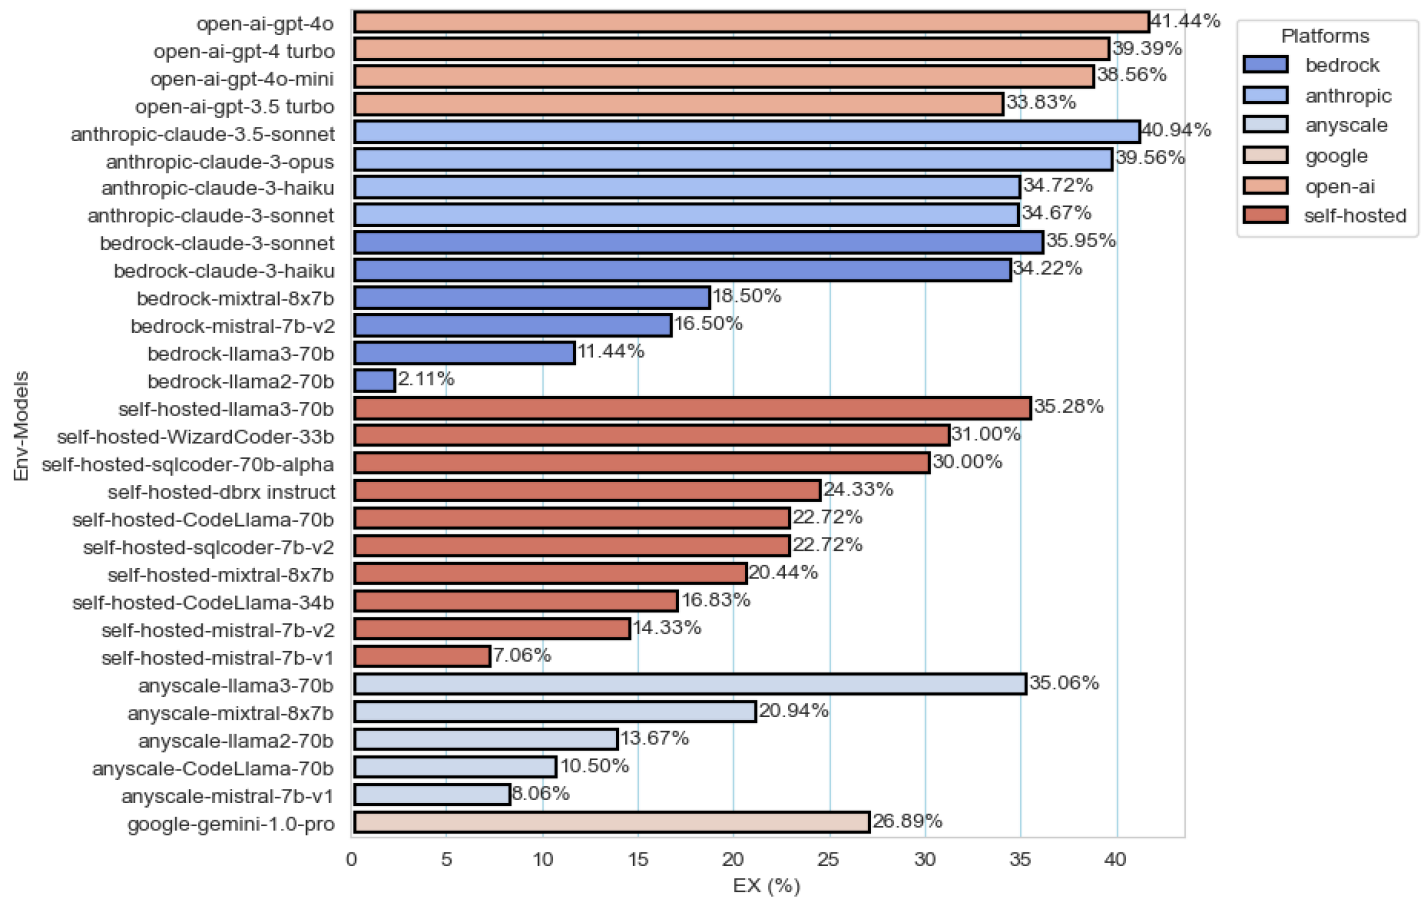
\includegraphics[width=0.8\textwidth]{rysunki/nltosql_dokladnosc_odpowiedzi.png}
        \captionof{figure}{ Dokładności modeli w zależności od platform hostujących w ramach benchmarku NL-to-SQL \cite{art3_structured2024}}
        \label{nltosql_dokladnosc_odpowiedzi}
    \end{center}

    \noindent Na następnym rysunku \ref{nltosql_koszt_odpowiedzi} przedstawiono średni koszt generowania odpowiedzi przez zewnętrznie hostowane modele w zależności od poziomu zaawansowania pytań. Model Claude3-Opus na platformie Anthropic okazał sie być najdroższym ze wszystkich modeli. Średni koszt wygenerowania wszystkich odpowiedzi w ramach testów wyniósł aż \$15.76. Jedynym darmowym modelem był Gemini 1.0 Pro, którego użycie skutkowało brakiem opłat za wygenerowanie wszystkich odpowiedzi. Z przytoczonych danych można wywnioskować, że wyższa cena modelu nie zawsze oznacza proporcjonalnie lepszą jakość.

    \begin{center}
        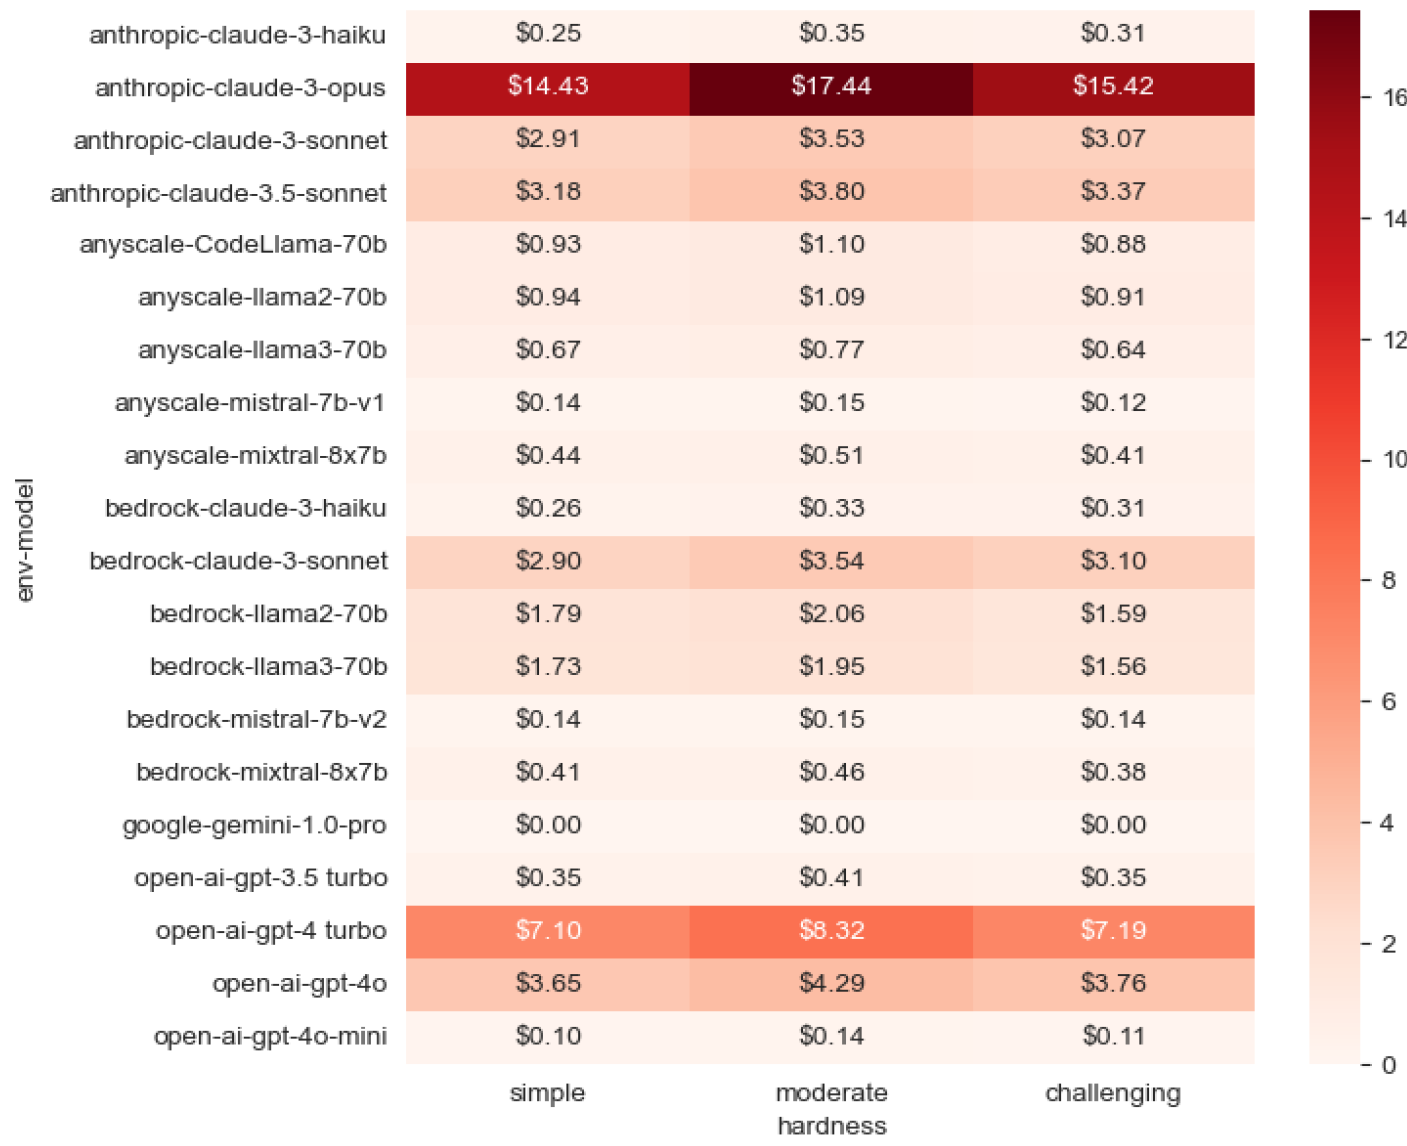
\includegraphics[width=0.7\textwidth]{rysunki/nltosql_koszt_odpowiedzi.png}
        \captionof{figure}{ Średnie koszty (w dolarze \$) generowania odpowiedzi dla zewnętrznie hostowanych modeli w zależności od stopnia zaawansowania pytań w ramach benchmarku NL-to-SQL \cite{art3_structured2024}}
        \label{nltosql_koszt_odpowiedzi}
    \end{center}

    \noindent Trzecim wartym uwagi wykresem jest ten wizualizujący średnią przepustowość modeli na wszystkich platformach w zależności od poziomu zaawansowania pytań \ref{nltosql_przepustowosc_modeli}. W tej kategorii najlepiej poradził sobie model Mistral-7B (Version 2) hostowany na platformie Amazon Bedrock. Jego średnia przepustowość wyniosła 87.11 t/s. Dla porównania, najmniejszą przepustowością wykazał się DBRX Instruct i wyniosła ona tylko 14.81 t/s.

    \begin{center}
        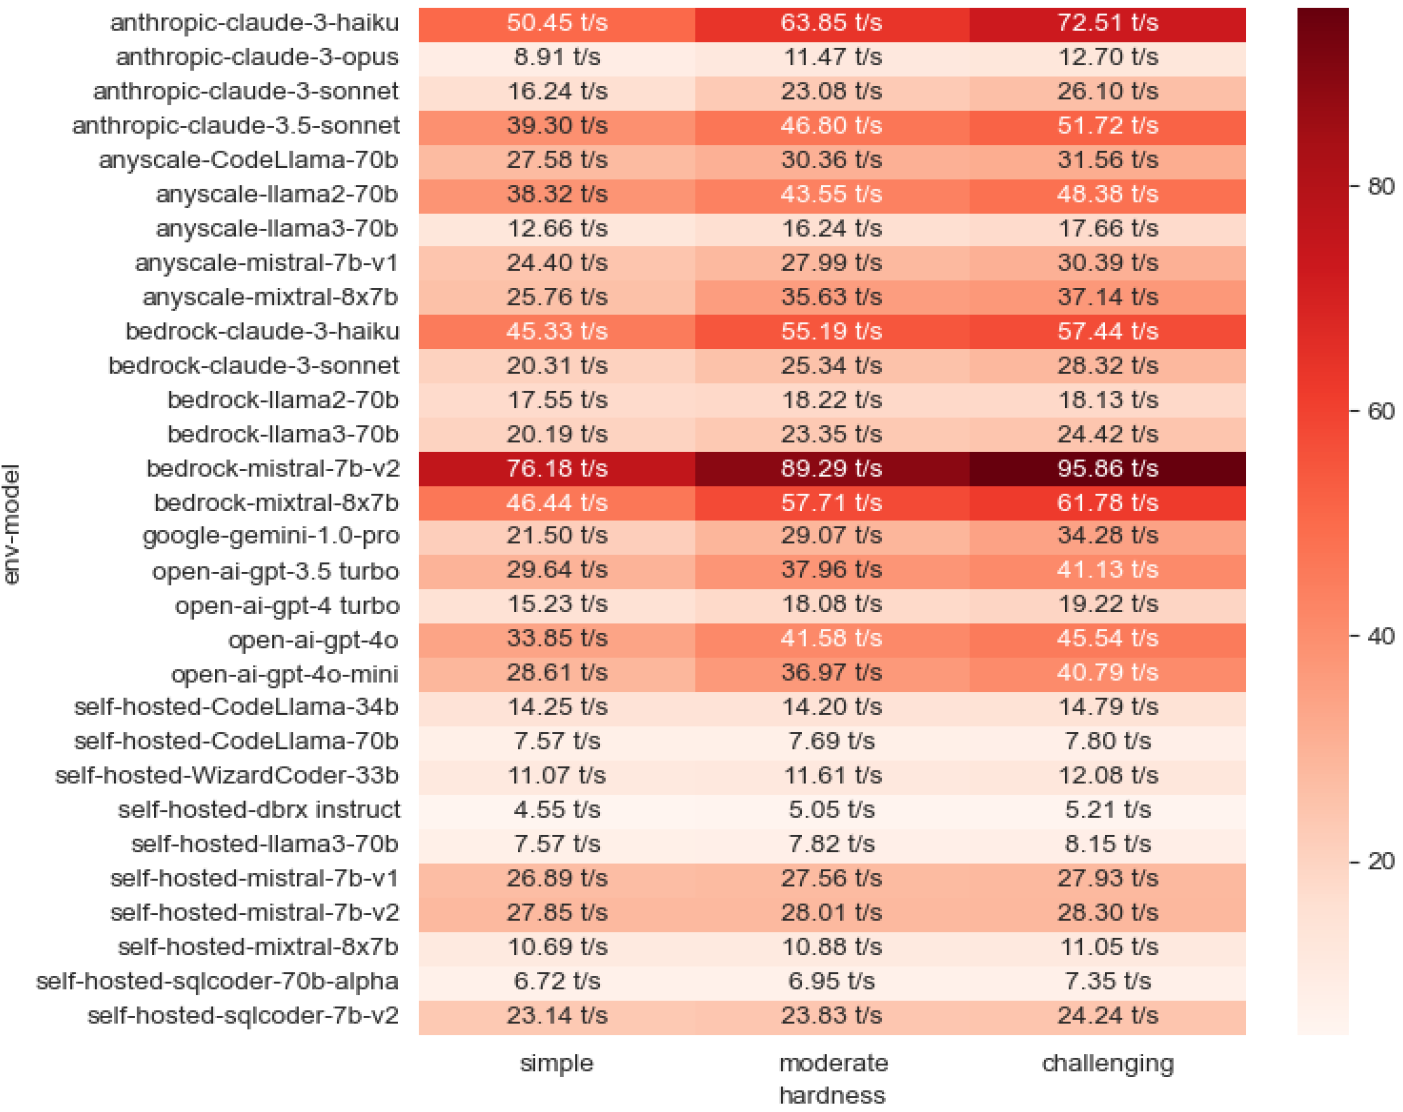
\includegraphics[width=0.7\textwidth]{rysunki/nltosql_przepustowosc_modeli.png}
        \captionof{figure}{ Średnie przepustowości (w tokenach na sekundę t/s) podczas generowania odpowiedzi dla wszystkich modeli w zależności od stopnia zaawansowania pytań w ramach benchmarku NL-to-SQL \cite{art3_structured2024}}
        \label{nltosql_przepustowosc_modeli}
    \end{center}

    \noindent Kompleksowe wyniki z artykułu wykazują, że wraz ze wzrostem trudności pytania, modelowi trudniej jest na nie trafnie odpowiedzieć. Co ciekawe, przepustowość rośnie proporcjonalnie do stopnia zaawansowania kwerendy. Najbardziej kosztowne okazało się generowanie odpowiedzi na średniozaawansowane pytania. Dalsze prace nad modelami LLM w zadaniach NL-to-SQL powinny koncentrować się na wdrażaniu technik few-shot learning, RAG i fine-tuningu oraz na optymalizacji wydajności i kosztów rozwiązań w ramach własnego hostingu.